\documentclass[conference]{IEEEtran}
\IEEEoverridecommandlockouts
\usepackage{cite}
\usepackage{amsmath,amssymb,amsfonts}
\usepackage{algorithmic}
\usepackage{graphicx}
\usepackage{textcomp}
\usepackage{xcolor}
\usepackage{tabularx}
\usepackage{booktabs}
\usepackage{tikz}
\usepackage{stfloats}
\usetikzlibrary{shapes.geometric, arrows.meta, positioning, fit}

\def\BibTeX{{\rm B\kern-.05em{\sc i\kern-.025em b}\kern-.08em
    T\kern-.1667em\lower.7ex\hbox{E}\kern-.125emX}}

\begin{document}

\title{Smart Parking Systems: A Comprehensive Review}

\author{\IEEEauthorblockN{1\textsuperscript{st} Ashutosh Sononey}
\IEEEauthorblockA{\textit{Computer Engineering} \\
\textit{FRCRCE}\\
Mumbai, India \\
ashutoshsononey@gmail.com}
}

\maketitle

\begin{abstract}
Rapid urbanization has significantly increased vehicle density across global metropolitan areas, leading to a severe parking shortage that exacerbates traffic congestion, environmental pollution, and substantial time loss for drivers. As cities transition toward smart infrastructure, traditional parking management proves insufficient. The objective of this paper is to comprehensively review the evolution and current state of smart parking technologies. The literature survey is systematically categorized into five technological layers: Traditional \& Spatial Management, Predictive AI \& Machine Learning, Blockchain \& Decentralized Networks, Dynamic Control via Reinforcement Learning, and Digital Twinning. By analyzing these layers, this review evaluates the main findings, highlights critical research gaps, and outlines the structural friction between digital simulation and physical deployment. Finally, we propose a conceptual hybrid architecture that integrates IoT sensors, machine learning predictions, blockchain allocation, and reinforcement learning to address the unresolved challenges in modern urban parking management.
\end{abstract}

\begin{IEEEkeywords}
smart parking, IOT sensors, digital twins, machine learning prediction, blockchain allocation, reinforcement learning
\end{IEEEkeywords}

\section{Introduction}

\subsection{Urban Parking Problem}
Large scale modern urbanisation and advent of modern cities strained the capacities of modern cities, many areas of cities suffering disproportionately than others. Lack of parking has been observed to bottleneck CBDs(Central business districts) maximum economic potential in the developing world. Vehicles cruising for parking are estimated to contribute to 30\% congestion within a transport network. Increasing noise, air pollution, and travel time delays. \cite{b12}. This cruising behavior to park vehicles wastes fuel, spikes carbon emissions, and in downstream has disproportionate economic impact, since transportation is a taut constraint for a variety of human markets.

\subsection{Traditional Parking Limitations}
Traditional parking management tends to consist of purely static approaches often involving supply chain maximization as informed by market economics. These have been varyingly successful compared to pure anarchy but, they frequently fail to be dynamic and adapt to changing environment often requiring government micro-management, as modern cities increase in size and scale this is going to be a persisting issue slowing down smart governance. Tradtitional system often fail to adjust price in real time, predict deman spikes and allocate sparse parking slots spatially leading to poor parking experience in diverse cosmopolitan cities\cite{b15}.

\subsection{Transition from Traditional to Smart Parking Systems}
Modern cities and municipalities in their jurisdictions are now actively trying to overcome these perils of traditional parking systems. They're deploying smart city initiatives, pertaining but not exclusive to smart parking systems, policies and citizen awareness. This transition from traditional parking involving manual painting parking spots to smart parking systems involving modern IOT sensors like RFID tags and fog computing \cite{b35}, deep learning computer vision \cite{b32}, to digital twinning for cyber-physical prediction of parking availability or multi-agent control systems\cite{b23}. This paper seeks to review these modern approaches.

\subsection{Research Gap}
Despite the various technological advancement in the field of smart parking, analysis of the literature suggests various research gaps. \textit{First}, many predictive AI models like RF perform well under controlled environment of studies but have difficulty with local volatility like weather or festivals if not accounted for during training\cite{b29}. \textit{Second}, hybrid or deep learning approaches like CatBoost are often understudied in the literature \cite{b32}. \textit{Third}, decentralized approaches presented in the research involving blockchain or alternatives find it difficult to scale\cite{b27}. \textit{Fourth}, AI based multi-agent routing or dynamic pricing is understudied field with sparse literature and often assume human drivers will behave rationally \cite{b23}. \textit{Fifth}, the up and coming digital twinning approaches struggle with an open-loop bottleneck i.e. they are incredible at predicting but lack autonomous physical control for dynamic pricing and feedback loop \cite{b1}. 

\subsection{Objective of this Paper}
This review presents a multi-layered classification of smart parking literature, categorizing the field into five distinct technological domains. We distill various methodologies, findings found in the literature and highlight research gap pertaining to each of the major approaches. Finally, we present a broad yet novel hybrid architecture which seeks to directionally aid the various bottlenecks and gaps overlooked in contemporary literature seeking to integrate IOT sensors, machine learning, blockchain ledgers, and reinforcement learning. 

\section{Technological Classification of Smart Parking Systems}
Following are the 5 major tiers using which the contemporary literature can be demarcated. This taxonomy contrasts earlier classical predictive approaches with more recent cyber-physical ones with various research progression in between. The field's general progression with increase in compute and data availability is towards the lower tiers:

\begin{itemize}
    \item \textbf{Traditional \& Spatial Management (The Physical Baseline):} Consists of geometric layout and markings, macro policies, and innovative deterministic non digital infrastructure.
    \item \textbf{Predictive AI \& Machine Learning (The Algorithmic Layer):} 
    This tier characterizes the short term and long term parking predictions using machine learning and deep learning tools/architectures such as ensembles and CNNs.
    \item \textbf{Blockchain \& Decentralized Networks (Trust vs. Throughput):} 
    Contains decentralized—cryptographic or non cryptographic approaches—to trustless parking allocations, mitigating single point of failures as well as addressing middle man. There's a recurring tradeoff between throughtput and trust.
    \item \textbf{Dynamic Control: Reinforcement Learning \& Multi-Agent Systems:}
    Focuses on dynamic price control and multi-agent predictive interventions in juxtaposition to traditional AI/ML.
    \item \textbf{Digital Twinning (The Cyber-Physical Frontier):} 
    Encompasses the emerging field of digital twinning and cyber physical systems, combining real-time spatial modelling with AI to simulate counterfactual urban scenarios in advanced.
\end{itemize}

Fig.~\ref{fig:taxonomy} depicts this categorical evolution.

\begin{figure}[!htbp]
\centering
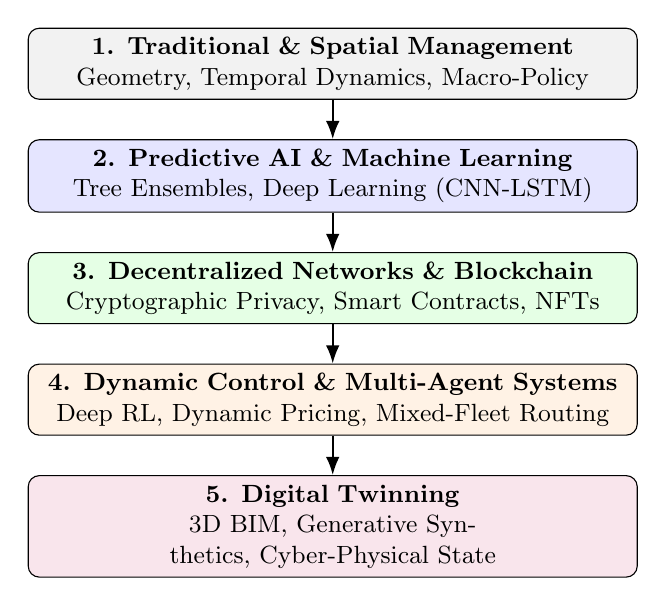
\begin{tikzpicture}[
    node distance=0.5cm and 0.5cm,
    box/.style={draw, rectangle, rounded corners, align=center, fill=blue!10, text width=7.5cm, font=\small, minimum height=0.8cm},
    arrow/.style={-Latex, thick}
]

\node (level1) [box, fill=gray!10] {\textbf{1. Traditional \& Spatial Management}\\Geometry, Temporal Dynamics, Macro-Policy};
\node (level2) [box, fill=blue!10, below=of level1] {\textbf{2. Predictive AI \& Machine Learning}\\Tree Ensembles, Deep Learning (CNN-LSTM)};
\node (level3) [box, fill=green!10, below=of level2] {\textbf{3. Decentralized Networks \& Blockchain}\\Cryptographic Privacy, Smart Contracts, NFTs};
\node (level4) [box, fill=orange!10, below=of level3] {\textbf{4. Dynamic Control \& Multi-Agent Systems}\\Deep RL, Dynamic Pricing, Mixed-Fleet Routing};
\node (level5) [box, fill=purple!10, below=of level4] {\textbf{5. Digital Twinning}\\3D BIM, Generative Synthetics, Cyber-Physical State};

\draw [arrow] (level1) -- (level2);
\draw [arrow] (level2) -- (level3);
\draw [arrow] (level3) -- (level4);
\draw [arrow] (level4) -- (level5);

\end{tikzpicture}
\caption{Taxonomy of Smart Parking Literature highlighting the technological evolution.}
\label{fig:taxonomy}
\end{figure}

\section{Traditional \& Spatial Management (The Physical Baseline)}
Foundational literature establishes the physical and geometric constraints of parking infrastructure. In terms of spatial layouts, discrete marking of parallel parking spaces has been shown to yield superior spatial utility compared to continuous, self-managed curb arrangements \cite{b24}. Furthermore, empirical observations in congested urban environments indicate a structural dominance of parallel parking over angular or perpendicular configurations, naturally occurring at a 2:1 ratio \cite{b9}. 

Analysis of temporal demand dynamics demonstrates severe variance based on infrastructure type and timing. Weekday peak durations are significantly extended for on-street parking, whereas weekend durations eclipse weekday peaks in terms of aggregate demand, particularly for off-street facilities \cite{b25}. Geographic Information System (GIS) regressions further validate that parking duration is not uniform, but rather categorically dictated by daily traffic volume, physical street length, and the existence of commercial land use (although limited by challenges such as obstructing tree canopies)\cite{b8}. Park-and-ride facility utilization similarly have strong temporal peaks on workdays, but the adoption rates are strictly bounded by the perceived reliability of associated public transit \cite{b37}.

Macro-level policy analyses have shifted towards highlighting systematic issues with supply-maximization strategies dominant in earlier literature. Transitioning to demand-side management—through cost internalization and shared use—can structurally reduce parking spatial requirements by 20–40\%, contingent on institutional friction \cite{b15}. The cascading externalities of on-street mismanagement are quantifiable; it directly contributes to traffic congestion and increases public bus scarcity by up to 38\% \cite{b17}. In contrast, the simulated implementation of structured multi-story facilities, demonstrates the capacity to double local travel speeds and reduce vehicular delays by 87\% \cite{b36}. Table~\ref{tab:traditional} summarizes the core literature in this domain.

\begin{table*}[!htbp]
\caption{Traditional \& Spatial Management Review}
\label{tab:traditional}
\centering
\begin{tabularx}{\textwidth}{@{} l >{\hsize=.15\hsize}X >{\hsize=.25\hsize}X >{\hsize=.3\hsize}X >{\hsize=.3\hsize}X @{}}
\toprule
\textbf{Ref.} & \textbf{Authors} & \textbf{Methodology} & \textbf{Key Findings} & \textbf{Research Gaps} \\
\midrule
\cite{b24} & Plasencia-Lozano et al. & Geometric occupancy analysis. & Discrete marking improves space utility. & Ignores large vehicles. \\
\cite{b9} & Olatunji et al. & Descriptive parking configuration analysis. & Parallel parking dominates (2:1). & Relies on slow government intervention. \\
\cite{b25} & Putri et al. & Cordon survey analysis. & Weekend durations exceed weekday peaks. & Omits probabilistic modeling. \\
\cite{b8} & Ajeng \& Gim & Regression with satellite/GIS. & Duration linked to volume \& commercial use. & Data fidelity issues (tree canopies). \\
\cite{b37} & Macioszek \& Kurek & Logit modeling of entry/exit. & Utilization peaks on workdays. & Excludes variables influencing adoption. \\
\cite{b15} & Chullabodhi et al. & Policy synthesis/taxonomic evaluation. & Demand-side management cuts space by 40\%. & Severe political friction. \\
\cite{b17} & Haider et al. & Mixed-methods qualitative/quantitative. & On-street parking increases bus scarcity by 38\%. & Lacks predictive frameworks. \\
\cite{b36} & Abood \& Khudhair & Simulation of multi-story interventions. & Structured parking slashes delays by 87\%. & Reliant on single dataset. \\
\bottomrule
\end{tabularx}
\end{table*}

\section{Predictive AI \& Machine Learning (The Algorithmic Layer)}
The field of predictive algorithms is a paradigmatic shift from descriptive statistics to probabilistic prediction. Within the domain of predictive AI/ML parking systems, tree-based ensembles, demonstrate high predictive power per cost. Random Forest (RF) and Decision Trees (DT) outperform alternative models (SVM,Naive Bayes, etc.) in precision and recall in predicting parking availability despite their vulnerability to unexpected local volatility and low computational overhead\cite{b21,b6,b29}. One major innovative approach used by Gomari et al \cite{b12} was to combine Parking Events (PE) features with ground truth data, a hybrid model of RF and XGBoost benefits from the respective advantages of each algorithm with minimal practical drawbacks, the use of PEs helped overcome RF's disadvantages by accounting for outliers dynamically. Channamallu et al. \cite{b14} highlight RF's ability capture variance introduced by localized anomalies, such as summer vacations or festivals, despite being unable to predict them without explicit training. Moreover, Gradient boosting frameworks like CatBoost achieve a 1.7\% predictive advantage over standard RF baselines by effectively integrating contextual urban data \cite{b10},an understudied model for parking prediction. 

To reduce system latency, researchers have deployed fog computing architectures combined with AdaBoost, which decreased response times compared to pure cloud based architectures \cite{b35}. Classical models have also proven effective when deployed on constrained edge hardware, such as Raspberry Pi integrated with OpenCV and ultrasonic sensors \cite{b28}, and in evaluating web-of-things datasets where RF showed strong temporal forecasting limits \cite{b30}. Simulator-based evaluations further provide evidence that RF and Artificial Neural Networks (ANN) have the high accuracy across multi-user behavioral archetypes \cite{b16}.

In contrast, forecasting complex, non-linear spatio-temporal conditions are better suited for Deep Learning architectures. Furthermore in a paper by google, parking difficult experienced by consumers of Google Maps was predicted using trajectory data which used double-layered Deep Neural Networks (DNN) and suggest that they generalize significantly better across major urban centers than single-layered regression models \cite{b18}. Consequently, a comprehensive 639 paper bibliometric review identifies a paradigmatic transition toward hybrid deep learning architectures—specifically CNN-LSTM networks—for processing multi-source image data \cite{b5}. While CNN-LSTM models demonstrate exceptional stability and accuracy in image-based free space detection \cite{b32}, they pose immense computational data requirements and exhibit high sensitivity to environmental noise, such as lighting fluctuations and are as such less feasible in their practical applications. Table~\ref{tab:ai_ml} details these algorithmic evaluations.

\begin{table*}[!htbp]
\caption{Predictive AI \& Machine Learning Review}
\label{tab:ai_ml}
\centering
\begin{tabularx}{\textwidth}{@{} l >{\hsize=.15\hsize}X >{\hsize=.25\hsize}X >{\hsize=.3\hsize}X >{\hsize=.3\hsize}X @{}}
\toprule
\textbf{Ref.} & \textbf{Authors} & \textbf{Methodology} & \textbf{Key Findings} & \textbf{Research Gaps} \\
\midrule
\cite{b21} & Dahiya et al. & IoT evaluation of KNN, SVM, RF, DT, LR, NB. & RF achieved superior precision. & Omits prediction transmission friction. \\
\cite{b6} & S. M.k. et al. & Prediction of sensor data (RF, KNN, LR). & RF proved most robust for length prediction. & Assumes stationary traffic distribution. \\
\cite{b29} & Dia et al. & Ensemble classifiers on 5M records. & Ensembles maximize validation scores. & Ignores local volatility (e.g., festivals). \\
\cite{b12} & Gomari et al. & Combinatorial ML (RF + XGBoost). & Optimal spatial forecasting via model fusion. & Excludes POI data due to uneven sets. \\
\cite{b14} & Channamallu et al. & Comparative modeling (RF, DT, SVR). & RF captures vacation/holiday variance. & Narrow scope (campus garages). \\
\cite{b10} & Jelen et al. & CRISP-DM evaluation (CatBoost vs RF). & CatBoost outperformed RF by 1.7\%. & Failed to incorporate POI variables. \\
\cite{b35} & Enríquez et al. & Fog architecture testing (AdaBoost, XGB). & Fog-cloud combinations reduced latency. & Lacks UI for real-time image status. \\
\cite{b28} & Singh et al. & Integration of Raspberry Pi \& OpenCV. & Frees street space via intelligent oversight. & Underspecified AI; lacks live prediction. \\
\cite{b30} & Provoost et al. & Measurement of NN, CNN, RF. & CNNs for short horizons; RF for longer. & Predictive horizon limited to 1 hour. \\
\cite{b16} & Bassetti et al. & Simulator of multi-user behavior. & RF and ANN provided highest accuracy. & Entirely reliant on simulated data. \\
\cite{b18} & Arora et al. & Double-layered DNN (Google Maps data). & DNN generalized better across cities. & Fails to account for seasonality. \\
\cite{b5} & Ma et al. & Bibliometric review of 639 articles. & Pivot toward hybrid deep learning (CNN-LSTM). & Over-indexes on deep learning. \\
\cite{b32} & Xu et al. & Space detection via CNN-LSTM. & Effectively captured spatio-temporal features. & Tested exclusively in sunny conditions. \\
\bottomrule
\end{tabularx}
\end{table*}

\section{Blockchain \& Decentralized Networks (Trust vs. Throughput)}
Decentralized networks have been proposed to address the single-point-of-failure vulnerabilities and lack of transparency associated with centralized cloud authorities. A primary objective within literature of this layer is cryptographic privacy. Deploying consortium blockchains integrated with Private Information Retrieval (PIR) protocols successfully obscures driver location data, mathematically decentralizing allocation while preventing lot favoritism \cite{b34}. At the edge layer, Raft consensus blockchains running on constrained IoT devices (e.g., Raspberry Pi) have demonstrated the capacity to execute cryptographic retrieval and reservation operations within microsecond margins \cite{b31}.

Limitations of many of proposed decentralized architectures lies in throughput bottlenecks and Oracle(a central source) reliance. A hybrid IoT deployment utilizing Ethereum smart contracts concluded that while decentralized ledgers successfully eliminate fixed server overhead during low-traffic periods, they cap at approximately 10 transactions per second (TPS), causing tremendous bottlenecks under high-velocity traffic compared to robust AWS cloud benchmarks which these approaches purport to challenge \cite{b27}. Furthermore, crowd-sourced parking pools monetized via Non-Fungible Tokens (NFTs) achieve trustless, tiered revenue sharing but relied on centralized government Oracles to verify physical land titles, fundamentally compromising the decentralized premise \cite{b26}. Post-blockchain federated architectures attempt to bypass transaction latency or time-to-finality by storing static data off-chain using IPFS (InterPlanteryFileSystem) and Zero-Knowledge Proofs, yet they empirically require fallback to centralized WebSockets to process high-frequency live physical state changes \cite{b39}. In small scale residential applications, AI-based systems bypass these ledger limitations entirely, utilizing standard architectures combined with GPS geo-fencing to achieve a 95\% sharing allocation rate \cite{b40}. Table~\ref{tab:blockchain} outlines the decentralization research.

\begin{table*}[!htbp]
\caption{Blockchain \& Decentralized Networks Review}
\label{tab:blockchain}
\centering
\begin{tabularx}{\textwidth}{@{} l >{\hsize=.15\hsize}X >{\hsize=.25\hsize}X >{\hsize=.3\hsize}X >{\hsize=.3\hsize}X @{}}
\toprule
\textbf{Ref.} & \textbf{Authors} & \textbf{Methodology} & \textbf{Key Findings} & \textbf{Research Gaps} \\
\midrule
\cite{b34} & Badr et al. & Consortium blockchain (PIR simulation). & Successfully decentralizes allocation. & Heavy PIR payloads risk high Gas costs. \\
\cite{b31} & Amiri et al. & Raft consensus blockchain (Raspberry Pi). & Microsecond cryptographic execution. & Conflates local speed with network latency. \\
\cite{b27} & Kalbhor et al. & YOLOv5 with Ethereum smart contracts. & Eliminates server overhead but caps at \~10 TPS. & Catastrophic throughput bottleneck. \\
\cite{b26} & Jennath et al. & IoT architecture monetizing land via NFTs. & Trustless, tiered revenue sharing. & Relies entirely on centralized Oracle. \\
\cite{b39} & Iacobescu et al. & Federated architecture (IPFS \& ZK Proofs). & Bypasses EVM latency off-chain. & Falls back to WebSockets for live data. \\
\cite{b40} & Hariharasudhan et al. & Mobile IoT with GPS geofencing \& RF. & Achieved 95\% allocation for sharing. & Limited to simulated data. \\
\bottomrule
\end{tabularx}
\end{table*}

\section{Dynamic Control: Reinforcement Learning \& Multi-Agent Systems}
Active intervention strategies can be found in the literature proposing Reinforcement Learning (RL) and multi-agent control systems to manipulate physical traffic flows dynamically. Automated dynamic pricing serves as the primary mechanism for demand distribution. \cite{b22} utilized a neural-network-based dynamic parking distribution model embedded with predictive control to establish a "sharing mode"—which actively routes overflow traffic to adjacent complementary facilities based on a multi-parameter utility function—significantly improves the resource utilization rate, effectively increasing overall system performance scores by 6–15\% compared to static, non-sharing modes.\cite{b11} implemented Deep Reinforcement Learning (DRL) algorithms (such as Q-learning) integrated with vehicle flow prediction successfully adjust hourly tariffs to spread out peak-hour vehicle flow, converging on frameworks that simultaneously maximize vendor revenue and regulate local traffic . Alternatively, localized deployments utilizing degree-4 polynomial regression provide a highly pragmatic software-layer predictive matrix that aligns dynamic tariffs closely with static baselines, outperforming heavier tree-based models locally \cite{b33}.

In the context of mixed-fleet environments, Multi-Agent Deep Reinforcement Learning (MARL) facilitates complex routing logic. By demarcating the environment into distinct agents, algorithms like QMIX can isolate the noise of unobservable Non-Connected Vehicles (NCVs). Dynamically routing only the Connected Vehicles (CVs) under the assumption of deterministic baseline behavioral logic reduces total systemic travel time by up to 15.7\% \cite{b23}. To provide the physical tracking for such routing, vision pipelines utilizing YOLOv5 achieve high accuracy (96.5\% mAP) on standard street-level data, though they suffer severe performance degradation when subjected to alternative aerial camera perspectives, indicating strong map-territory conflation \cite{b7}. Table~\ref{tab:dynamic_rl} reviews the active control systems.

\begin{table*}[!htbp]
\caption{Dynamic Control \& Reinforcement Learning Review}
\label{tab:dynamic_rl}
\centering
\begin{tabularx}{\textwidth}{@{} l >{\hsize=.15\hsize}X >{\hsize=.25\hsize}X >{\hsize=.3\hsize}X >{\hsize=.3\hsize}X @{}}
\toprule
\textbf{Ref.} & \textbf{Authors} & \textbf{Methodology} & \textbf{Key Findings} & \textbf{Research Gaps} \\
\midrule
\cite{b22} & Zhao et al. & Neural-network Model Predictive Control. & Routing overflow improves system by 6-15\%. & Relies on fixed fees. \\
\cite{b11} & Poh et al. & Deep RL (Q-learning) with flow prediction. & DRL dynamic pricing disperses peak flow. & Ignores on-street parking alternatives. \\
\cite{b33} & Raghuraman et al. & Degree-4 polynomial regression. & Outperforms heavier tree-based models locally. & Functions as software matrix without IoT. \\
\cite{b23} & Zhang et al. & Multi-Agent Deep RL (MARL). & Routing Connected Vehicles cuts travel time 15.7\%. & Assumes perfect FCFS logic for users. \\
\cite{b7} & Leng \& Guo & Blockchain/IoT pipeline (YOLOv5). & Achieves 96.5\% mAP on street-level data. & Severe map-territory conflation. \\
\bottomrule
\end{tabularx}
\end{table*}

\section{Digital Twinning (The Cyber-Physical Frontier)}
Digital Twin (DT) approach for parking prediction is the intersection of spatial modeling and real-time prediction, yet the literature persistently elucidates the structural friction between digital simulation and practical physical deployment. The spatial fidelity of a DT dictates its specific hardware vulnerabilities. Basic 2D IoT deployments utilizing dual-ultrasonic sensors provide highly accurate (99.63\%) state reflection to cloud dashboards with minimal false positives due to their structural simplicity \cite{b3}. In contrast, high-fidelity 3D Building Information Modelling (BIM) twins integrated with real-time object detection (e.g. YOLOv3/v7) provide more accurate spatial visualization but expose many hardware flaws such as: low-FPS cameras, sunlight glare, and pedestrian occlusion cause severe motion blur, repeatedly disrupting License Plate Recognition (LPR) algorithms and corrupting occupancy counts \cite{b2,b13}.

To combine static models with dynamic urban planning, recent literature uses generative AI. These advanced frameworks proactively generate counterfactual realities. A flagship example is the comprehensive digital twin framework proposed by Piccialli et al., which integrates predictive modeling (using Spatial-Temporal Identity networks) with a generative simulation engine (CVAE-WGAN) \cite{b1}. Validated using real-world data from Caserta, Italy, this three-tier architecture allows policymakers to synthesize highly realistic counterfactual scenarios (eg; sudden zone closures, severe weather impacts, or the construction of multi-story facilities) before committing physical resources \cite{b1,b20}.

Yet drawbacks remain, the literature acknowledges a persistent "open-loop" execution bottleneck. Despite using advanced 3D Unity modeling, LSTM forecasting, Full Velocity Difference Models (FVDM), and Particle Swarm Optimization \cite{b19,b4,b38} or structured feedback loops through periodic model retraining \cite{b1}. Many of them operate as decision-support dashboards with a human-in-the-loop (HIIT) required. Further research is necessary to reduce human involvement within the system.
Table~\ref{tab:digital_twin} synthesizes these methodologies.

\begin{table*}[!htbp]
\caption{Digital Twinning Review}
\label{tab:digital_twin}
\centering
\begin{tabularx}{\textwidth}{@{} l >{\hsize=.15\hsize}X >{\hsize=.25\hsize}X >{\hsize=.3\hsize}X >{\hsize=.3\hsize}X @{}}
\toprule
\textbf{Ref.} & \textbf{Authors} & \textbf{Methodology} & \textbf{Key Findings} & \textbf{Research Gaps} \\
\midrule
\cite{b2} & Zou et al. & Digital Twin fusing YOLOv3 with BIM. & Dual-sensor minimizes false positives (99.63\%). & Limited to 2D layout; lacks structural depth. \\
\cite{b13} & Coching et al. & 3D BIM DT with YOLOv7 (LPR). & Intuitive 3D visualization (~95\% accuracy). & Low-FPS cameras disrupted LPR. \\
\cite{b3} & Amusan \& Ogunleye & IoT deployment (ultrasonic + Firebase). & Reflects physical changes in real-time. & Emission reductions theoretically projected. \\
\cite{b20} & Canzaniello et al. & DT framework integrating LSTM and GAN. & Synthetics align with real-world dynamics. & Epistemic looping via artificial realities. \\
\cite{b1} & Piccialli et al. & 3-tier DT (STID prediction, CVAE-WGAN). & Validated generative what-if scenario forecasting. & Lacks automated feedback loop for real-time actuation. \\
\cite{b19} & Chen et al. & DT (Unity 3D, LSTM, Velocity Model). & Dynamic spatial planning maximizes safety. & Tailored to specific residential geometries. \\
\cite{b4} & Sahu et al. & Hybrid edge-cloud simulating Pareto optimization. & 25\% faster search and 30\% less congestion. & Relies on synthetic distributions. \\
\cite{b38} & Chomiak-Orsa et al. & DT simulation (Flexsim) via open-data. & Visualizes occupancy mirroring routine behaviors. & Fails to model turbulent environmental anomalies. \\
\bottomrule
\end{tabularx}
\end{table*}

\section{Research Challenges and Open Issues}
As per the contemporary literature, several major hurdles are blocking the deployment of fully autonomous smart parking: 


First, \textit{Data Fidelity and Hardware Vulnerability}, High-fidelity 3D Digital Twins and computer vision approaches (eg; YOLOv5, CNN-LSTM) fail to extrapolate when exposed to real-world environmental noise (eg; bad camera angle, low framerates et cetra) \cite{b7,b13}. 

Second, the \textit{Throughput versus Trust} tradeoff in decentralized systems. Blockchain based architectures that attempt to eliminate central cloud costs usually tradeoff decentralization for low transaction rates (eg; 10 TPS), making them impractical for volumetrically dense city traffic without falling back on centralized services like AWS \cite{b27,b39}. 

Third, \textit{Behavioral Friction} constantly disrupts algorithmic efficiency. Multi-agent routing algorithms and predictive models usually rely on strict deterministic assumptions, completely ignoring the irrational preferences of human drivers or unpredictable local events \cite{b23,b29}. The surveyed literature on multi-agent or RL doesn't predominantly use AI for smart parking systems; this is one area which can be further explored. 

Finally, the \textit{Open-Loop Execution Bottleneck} is one of the major reasons plaguing digital twin-based approaches. Modern cyber-physical systems can synthesize data and simulate complex pricing models when provided with high-quality data, but they lack the autonomous physical capability to enforce those decisions in real-time. They still require a human in the loop to pull the lever \cite{b1,b20}.

\section{Proposed Hybrid Architecture}
To bridge the gaps left by isolated technologies, we outline a conceptual hybrid architecture that pulls together IoT, Machine Learning, Blockchain, and Reinforcement Learning into a single, cohesive loop.

At the physical edge, an \textit{IoT Sensor Network} tracks real-time spatial occupancy. To overcome the environmental vulnerabilities of computer vision identified in the literature, this layer relies on dual-sensor confirmation (pairing robust ultrasonic sensors with lightweight vision) to eliminate false positives caused by weather or lighting \cite{b2,b3}. This live feed pushes directly into the \textit{Machine Learning Prediction Layer}, where tree-based ensembles like Random Forest combined with XGBoost utilize extracted Parking Events (PE) features alongside real-time ground truth data to anticipate short-term availability and adjust for local temporal variance \cite{b12}.

Rather than having a single point of failure, allocation and financial transactions shift to a \textit{Blockchain Allocation Layer}. By keeping static data off-chain (via IPFS) and running lightweight smart contracts, the system provides trustless revenue sharing for commercial and residential pools without triggering the severe throughput bottlenecks seen in pure on-chain deployments \cite{b39,b40}.

To close the execution loop, the \textit{Reinforcement Learning Dynamic Control Layer} is implemented to account for human behavioral friction, the system utilizes Multi-Agent Deep RL to manage a mixed-fleet environment,dynamically routing predictable CVs (Connected Vehicles) to underutilized facilities to offset the unpredictable noise of human drivers \cite{b23}. Furthermore, this layer directly solves the open-loop bottleneck by bypassing human operators entirely; the RL algorithm is directly integrated with physical IoT actuators, such as automated smart-barriers and real-time digital pricing boards, transforming passive digital twin observations into automated, system-wide physical actuation \cite{b11,b22}.

\section{Conclusion}
This paper reviewed the relatively young field of smart parking systems, demarcating the literature into five distinct layers : Traditional Management, Predictive AI, Decentralized Networks, Dynamic Control, and Digital Twinning. 

Although moving from basic spatial management to complex cyber-physical abstractions has given us predictive power, many research gaps remain. The friction between clean digital simulations and a capricious physical world (Eg; hardware vulnerabilities, blockchain throughput bottlenecks, or RL agentic frameworks assuming drivers act like perfectly rational agents) hinders the current systems from achieving widespread adoption. The persistent open-loop bottleneck in many digital twinning studies means even the most advanced frameworks today are predictive rather than dynamic and sensitive to adjusting pricing and market forces. To address this, the paper proposed a broad hybrid architecture that combines data from IoT sensors, uses machine learning for predictions,blockchain to avoid centralization and RL for dynamic pricing. Future research, can focus on addressing the cyber-physical loop, building systems that can autonomously adapt to the chaotic, high-velocity reality of urban traffic, and more AI RL dynamic pricing based architectures to contrast with established ones.
\begin{thebibliography}{00}
\bibitem{b1} F. Piccialli, S. Amitrano, D. Cerciello, A. Borrelli, E. Prezioso, and M. Canzaniello, “A digital twin framework for urban parking management and mobility forecasting,” Nat Commun, vol. 16, no. 1, p. 9400, Oct. 2025, doi: 10.1038/s41467-025-65306-w.
\bibitem{b2} Y. Zou, F. Ye, A. Li, M. Munir, E. Hjelseth, and S. F. Sujan, “A Digital Twin prototype for smart parking management,” in ECPPM 2022 - eWork and eBusiness in Architecture, Engineering and Construction 2022, CRC Press, 2023.
\bibitem{b3} A. A. Amusan and G. A. Ogunleye, “A Digital Twin-Enabled Smart Car Park Management System: Architecture and Impact on Emission Reduction,” FUOYE Journal of Engineering and Technology, vol. 9, no. 4, pp. 629–635, 2024, doi: 10.4314/fuoyejet.v9i4.10.
\bibitem{b4} D. Sahu, P. Sinha, S. Prakash, T. Yang, R. S. Rathore, and L. Wang, “A multi objective optimization framework for smart parking using digital twin pareto front MDP and PSO for smart cities,” Sci Rep, vol. 15, no. 1, p. 7783, Mar. 2025, doi: 10.1038/s41598-025-91565-0.
\bibitem{b5} C. Ma, X. Huang, and J. Li, “A review of research on urban parking prediction,” Journal of Traffic and Transportation Engineering (English Edition), vol. 11, no. 4, pp. 700–720, Aug. 2024, doi: 10.1016/j.jtte.2023.11.004.
\bibitem{b6} S. M.k., H. J., K. S. Santhosh Kumar, and S. P. Shiva Prakash, “AI-Powered Hybrid Smart Parking: Optimizing Parking Management Across Diverse Applications in Smart Cities,” Procedia Computer Science, vol. 258, pp. 1524–1535, Jan. 2025, doi: 10.1016/j.procs.2025.04.385.
\bibitem{b7} J. Leng and Y. Guo, “AI-Powered Smart Parking Management: Optimizing Allocation and Safety,” in Proceedings of the 2024 8th International Conference on Big Data and Internet of Things, in BDIOT ’24. New York, NY, USA: Association for Computing Machinery, Dec. 2024, pp. 397–403. doi: 10.1145/3697355.3697421.
\bibitem{b8} C. Ajeng and T.-H. T. Gim, “Analyzing on-Street Parking Duration and Demand in a Metropolitan City of a Developing Country: A Case Study of Yogyakarta City, Indonesia,” Sustainability, vol. 10, no. 3, p. 591, Mar. 2018, doi: 10.3390/su10030591.
\bibitem{b9} A. Olatunji, E. John, A. Adedeji, and M. Mikaila, “Assessment of Parking Facilities in Public Areas: The Case of Keffi Town,” CSID Journal of Infrastructure Development, vol. 7, no. 3, Dec. 2024, doi: 10.7454/jid.v7.i3.1152.
\bibitem{b10} G. Jelen, V. Podobnik, and J. Babic, “Contextual prediction of parking spot availability: A step towards sustainable parking,” Journal of Cleaner Production, vol. 312, p. 127684, Aug. 2021, doi: 10.1016/j.jclepro.2021.127684.
\bibitem{b11} L. Z. Poh, T. Connie, T. S. Ong, and M. K. O. Goh, “Deep Reinforcement Learning-Based Dynamic Pricing for Parking Solutions,” Algorithms, vol. 16, no. 1, p. 32, Jan. 2023, doi: 10.3390/a16010032.
\bibitem{b12} S. Gomari, R. Domakuntla, C. Knoth, and C. Antoniou, “Development of a Data-Driven On-Street Parking Information System Using Enhanced Parking Features,” IEEE Open Journal of Intelligent Transportation Systems, vol. 4, pp. 30–47, 2023, doi: 10.1109/OJITS.2023.3235898.
\bibitem{b13} J. K. Coching, R. K. C. Billones, A. K. M. Brillantes, S. Yunus, V. A. Pitogo, and R. Senkerik, “Digital Twinning Mechanism and Building Information Modeling for a Smart Parking Management System,” Smart Cities, vol. 8, no. 5, p. 146, Oct. 2025, doi: 10.3390/smartcities8050146.
\bibitem{b14} S. S. Channamallu, V. K. Padavala, S. Kermanshachi, J. M. Rosenberger, and A. Pamidimukkala, “Examining parking occupancy prediction models: a comparative analysis,” Transportation Research Procedia, vol. 73, pp. 281–288, Jan. 2023, doi: 10.1016/j.trpro.2023.11.919.
\bibitem{b15} C. Chullabodhi, S. Chalermpong, and A. Ratanawaraha, “Examining the Root Causes of On-Street Parking Mismanagement in Central Bangkok,” Nakhara: Journal of Environmental Design and Planning, vol. 21, no. 1, pp. 207–207, Jun. 2022, doi: 10.54028/NJ202221207.
\bibitem{b16} E. Bassetti, A. Berti, A. Bisante, A. Magnante, and E. Panizzi, “Exploiting User Behavior to Predict Parking Availability through Machine Learning,” Smart Cities, vol. 5, no. 4, pp. 1243–1266, Dec. 2022, doi: 10.3390/smartcities5040064.
\bibitem{b17} M. A. Haider, M. T. Islam, and S. M. Hasan, “Exploring the Impact of On-street Parking in Chittagong City, Bangladesh,” International Journal of Building, Urban, Interior and Landscape Technology, vol. 17, pp. 17–28, Jun. 2021.
\bibitem{b18} N. Arora et al., “Hard to Park? Estimating Parking Difficulty at Scale,” in Proceedings of the 25th ACM SIGKDD International Conference on Knowledge Discovery \& Data Mining, in KDD ’19. New York, NY, USA: Association for Computing Machinery, Jul. 2019, pp. 2296–2304. doi: 10.1145/3292500.3330767.
\bibitem{b19} W. Chen, X. Wang, and M. Wu, “Intelligent Parking Service System Design Based on Digital Twin for Old Residential Areas,” Electronics, vol. 13, no. 23, p. 4597, Jan. 2024, doi: 10.3390/electronics13234597.
\bibitem{b20} M. Canzaniello, S. Amitrano, E. Prezioso, F. Giampaolo, S. Cuomo, and F. Piccialli, “Leveraging Digital Twins and Generative AI for Effective Urban Mobility Management,” in 2024 IEEE Cyber Science and Technology Congress (CyberSciTech), Nov. 2024, pp. 146–153. doi: 10.1109/CyberSciTech64112.2024.00032.
\bibitem{b21} A. Dahiya et al., “Machine Learning-Based Prediction of Parking Space Availability in IoT-Enabled Smart Parking Management Systems,” Journal of Advanced Transportation, vol. 2024, no. 1, p. 8474973, 2024, doi: 10.1155/2024/8474973.
\bibitem{b22} Z. Zhao, Y. Zhang, K. Ji, and H. Qi, “Neural-Network-Based Dynamic Distribution Model of Parking Space Under Sharing and Non-Sharing Modes,” Sustainability, vol. 12, no. 12, p. 4864, Jan. 2020, doi: 10.3390/su12124864.
\bibitem{b23} X. Zhang, C. Zhao, F. Liao, X. Li, and Y. Du, “Online parking assignment in an environment of partially connected vehicles: A multi-agent deep reinforcement learning approach,” Transportation Research Part C: Emerging Technologies, vol. 138, p. 103624, May 2022, doi: 10.1016/j.trc.2022.103624.
\bibitem{b24} P. Plasencia-Lozano and I. Méndez-Manjón, “Optimisation of urban space based on geometric analysis of parallel parking lots,” Transportation Research Procedia, vol. 71, pp. 307–314, Jan. 2023, doi: 10.1016/j.trpro.2023.11.089.
\bibitem{b25} D. A. P. A. G. Putri, P. Nadun, I. Kumara, and D. Indrashwara, “Optimizing Public Parking System at Traditional Market,” Jurnal Teknik Sipil, vol. 24, pp. 1523–1531, Jan. 2025, doi: 10.26418/jts.v24i4.86617.
\bibitem{b26} H. S. Jennath, S. Adarsh, N. V. Chandran, R. Ananthan, A. Sabir, and S. Asharaf, “Parkchain: A Blockchain Powered Parking Solution for Smart Cities,” Front. Blockchain, vol. 2, Aug. 2019, doi: 10.3389/fbloc.2019.00006.
\bibitem{b27} A. Kalbhor et al., “PARKTag: An AI–Blockchain Integrated Solution for an Efficient, Trusted, and Scalable Parking Management System,” Technologies, vol. 12, no. 9, p. 155, Sep. 2024, doi: 10.3390/technologies12090155.
\bibitem{b28} T. Singh, R. Rathore, K. Gupta, E. Vijay, and R. Harikrishnan, “(PDF) Artificial Intelligence-Enabled Smart Parking System,” ResearchGate, doi: 10.1007/978-981-99-8661-3\_31.
\bibitem{b29} I. Dia, E. Ahvar, and G. M. Lee, “Performance Evaluation of Machine Learning and Neural Network-Based Algorithms for Predicting Segment Availability in AIoT-Based Smart Parking,” Network, vol. 2, no. 2, pp. 225–238, Jun. 2022, doi: 10.3390/network2020015.
\bibitem{b30} J. C. Provoost, A. Kamilaris, L. J. J. Wismans, S. J. van der Drift, and M. van Keulen, “Predicting parking occupancy via machine learning in the web of things,” Internet of Things, vol. 12, p. 100301, Dec. 2020, doi: 10.1016/j.iot.2020.100301.
\bibitem{b31} W. A. Amiri, M. Baza, K. Banawan, M. Mahmoud, W. Alasmary, and K. Akkaya, “Privacy-Preserving Smart Parking System Using Blockchain and Private Information Retrieval,” in 2019 International Conference on Smart Applications, Communications and Networking (SmartNets), Dec. 2019, pp. 1–6. doi: 10.1109/SmartNets48225.2019.9069783.
\bibitem{b32} Z. Xu, X. Tang, C. Ma, and R. Zhang, “Research on Parking Space Detection and Prediction Model Based on CNN-LSTM,” IEEE Access, vol. 12, pp. 30085–30100, 2024, doi: 10.1109/ACCESS.2024.3368521.
\bibitem{b33} G. Raghuraman, S. Kavitha, N. Gokulakrishnan, S. Radhakrishnan, and P. Ramakrishnan, “Smart Parking System with Dynamic Pricing Model,” INDJST, vol. 16, no. 18, pp. 1332–1339, May 2023, doi: 10.17485/IJST/v16i18.2489.
\bibitem{b34} M. M. Badr, W. A. Amiri, M. M. Fouda, M. M. E. A. Mahmoud, A. J. Aljohani, and W. Alasmary, “Smart Parking System With Privacy Preservation and Reputation Management Using Blockchain,” IEEE Access, vol. 8, pp. 150823–150843, 2020, doi: 10.1109/ACCESS.2020.3016945.
\bibitem{b35} F. J. Enríquez, J.-M. Mejía-Muñoz, G. Bravo, and O. Cruz-Mejía, “Smart Parking: Enhancing Urban Mobility with Fog Computing and Machine Learning-Based Parking Occupancy Prediction,” Applied System Innovation, vol. 7, no. 3, p. 52, Jun. 2024, doi: 10.3390/asi7030052.
\bibitem{b36} S. S. Abood and H. A. Khudhair, “The Impact of Multi-Story Parking Facilities on Traffic Flow: The Case Study of the Al-Maidan Area in Baghdad City,” Engineering, Technology \& Applied Science Research, vol. 15, no. 5, pp. 26908–26916, Oct. 2025, doi: 10.48084/etasr.12678.
\bibitem{b37} E. Macioszek and A. Kurek, “The Use of a Park and Ride System—A Case Study Based on the City of Cracow (Poland),” Energies, vol. 13, no. 13, p. 3473, Jan. 2020, doi: 10.3390/en13133473.
\bibitem{b38} I. Chomiak-Orsa, K. Hauke, K. Perechuda, and M. Pondel, “The use of Digital Twin in the sustainable development of the city on the example of managing parking resources,” Procedia Computer Science, vol. 225, pp. 2183–2193, Jan. 2023, doi: 10.1016/j.procs.2023.10.209.
\bibitem{b39} C. Iacobescu, G. Oltean, C. Florea, and B. Burtea, “Unified InterPlanetary Smart Parking Network for Maximum End-User Flexibility,” Sensors, vol. 22, no. 1, p. 221, Jan. 2022, doi: 10.3390/s22010221.
\bibitem{b40} S. Hariharasudhan, R. Karthika, K. Malarvizhi, P. S. Rekha, D. Vikram, and S. P. Santhoshkumar, “Urban ParkAI: An AI-based Residential Parking Management System for Smart City Planning,” in 2025 5th International Conference on Ubiquitous Computing and Intelligent Information Systems (ICUIS), Nov. 2025, pp. 772–777. doi: 10.1109/ICUIS67429.2025.11380472.
\end{thebibliography}
\end{document}
